%% 
%% Copyright 2007, 2008, 2009 Elsevier Ltd
%% 
%% This file is part of the 'Elsarticle Bundle'.
%% ---------------------------------------------
%% 
%% It may be distributed under the conditions of the LaTeX Project Public
%% License, either version 1.2 of this license or (at your option) any
%% later version.  The latest version of this license is in
%%    http://www.latex-project.org/lppl.txt
%% and version 1.2 or later is part of all distributions of LaTeX
%% version 1999/12/01 or later.
%% 
%% The list of all files belonging to the 'Elsarticle Bundle' is
%% given in the file `manifest.txt'.
%% 

%% Template article for Elsevier's document class `elsarticle'
%% with numbered style bibliographic references
%% SP 2008/03/01

\documentclass[preprint,12pt, a4paper]{elsarticle}

%% Use the option review to obtain double line spacing
%% \documentclass[authoryear,preprint,review,12pt]{elsarticle}

%% For including figures, graphicx.sty has been loaded in
%% elsarticle.cls. If you prefer to use the old commands
%% please give \usepackage{epsfig}

%% The amssymb package provides various useful mathematical symbols
\usepackage{amssymb}
%% The amsthm package provides extended theorem environments
%% \usepackage{amsthm}

%% The lineno packages adds line numbers. Start line numbering with
%% \begin{linenumbers}, end it with \end{linenumbers}. Or switch it on
%% for the whole article with \linenumbers.
\usepackage{lineno}

\usepackage{float}
\restylefloat{table}

\journal{SoftwareX}

\begin{document}

\begin{frontmatter}

%% Title, authors and addresses

%% use the tnoteref command within \title for footnotes;
%% use the tnotetext command for theassociated footnote;
%% use the fnref command within \author or \address for footnotes;
%% use the fntext command for theassociated footnote;
%% use the corref command within \author for corresponding author footnotes;
%% use the cortext command for theassociated footnote;
%% use the ead command for the email address,
%% and the form \ead[url] for the home page:
%% \title{Title\tnoteref{label1}}
%% \tnotetext[label1]{}
%% \author{Name\corref{cor1}\fnref{label2}}
%% \ead{email address}
%% \ead[url]{home page}
%% \fntext[label2]{}
%% \cortext[cor1]{}
%% \address{Address\fnref{label3}}
%% \fntext[label3]{}

\title{Title/Name of your software}

%% use optional labels to link authors explicitly to addresses:
%% \author[label1,label2]{}
%% \address[label1]{}
%% \address[label2]{}

\author{A. Author}

\address{Your institute, some address}

\begin{abstract}
%% Text of abstract 
Ca. 100 words

\end{abstract}

\begin{keyword}
%% keywords here, in the form: keyword \sep keyword
keyword 1 \sep keyword 2 \sep keyword 3

%% PACS codes here, in the form: \PACS code \sep code

%% MSC codes here, in the form: \MSC code \sep code
%% or \MSC[2008] code \sep code (2000 is the default)

\end{keyword}

\end{frontmatter}

\section*{Required Metadata}
\label{}

\section*{Current code version}
\label{}

Ancillary data table required for subversion of the codebase. Kindly replace examples in right column with the correct information about your current code, and leave the left column as it is.

\begin{table}[H]
\begin{tabular}{|l|p{6.5cm}|p{6.5cm}|}
\hline
\textbf{Nr.} & \textbf{Code metadata description} & \textbf{Please fill in this column} \\
\hline
C1 & Current code version & For example v42 \\
\hline
C2 & Permanent link to code/repository used for this code version & For example: $https://github.com/mozart/mozart2$ \\
\hline
C3 & Code Ocean compute capsule & For example: $https://codeocean.com/2017/07/30/neurospeech-colon-an-open-source-software-for-parkinson-apos-s-speech-analysis/code$\\
\hline
C4 & Legal Code License   & List one of the approved licenses \\
\hline
C5 & Code versioning system used & For example svn, git, mercurial, etc. put none if none \\
\hline
C6 & Software code languages, tools, and services used & For example C++, python, r, MPI, OpenCL, etc. \\
\hline
C7 & Compilation requirements, operating environments \& dependencies & \\
\hline
C8 & If available Link to developer documentation/manual & For example: $http://mozart.github.io/documentation/$ \\
\hline
C9 & Support email for questions & \\
\hline
\end{tabular}
\caption{Code metadata (mandatory)}
\label{} 
\end{table}

%% main text

The permanent link to code/repository or the zip archive should include the following requirements: 

README.txt and LICENSE.txt.

Source code in a src/ directory, not the root of the repository.

Tag corresponding with the version of the software that is reviewed.

Documentation in the repository in a docs/ directory, and/or READMEs, as appropriate.

\linenumbers

\section{Motivation and significance}
\label{motivation}

Development efforts for UI libraries and frameworks dedicated to desktop and workstation software
have virtually stalled compared with modern web UI frameworks. User expectations for most software
packages center on one experience: is the software available as a reactive web or mobile
application? The interest in such a deployment mechanism comes from the convenience of immediate use
and the lack of any installation time or maintenance. 

The same preferences can be found with users of neutron scattering facilities—such as HFIR and
SNS—who have significantly compressed schedules during their visits. The demands of their
experiments leave little time for complicated software and installation procedures. Furthermore,
when these users return to their institutions, debugging remote issues on native desktop software
can be extremely time consuming, if not impossible, for the development team. In contrast to their
native counterparts, web UIs have no installation time, and problems are relatively easy to diagnose
remotely. Web UIs also have the added benefit of central deployment in which fixing a bug for one
user immediately fixes the bug for all users (to within cache refresh times).

Shaman is a new web interface for data reduction for the Bio-SANS, EQ-SANS, and GP-SANS instruments
at HFIR and SNS. Fundamental goals of its development include quick turnaround for users and easy
access to data. This includes streamlining the workflow to quickly and reactively prepare the
reduction configuration needed to reduce the data, as well as integrated interactive visualization
and data export tools for working with that data. The user experience across all three instruments
is the same with identification of the specific instrument required only for gathering the correct
data and launching the correct reduction program on the server. 
\section{Software description}
\label{description}

The primary workflow of Shaman begins with user authentication and instrument selection. Once the
instrument is selected, users are presented with the list of experiments associated with their
account in a proposal tracking system. Experiment selection is followed by parameter configuration
and the selection of individual runs from the experiment that will be used as part of the reduction.
Each run is further distinguished by the order in which it should be reduced and whether or not the
output of reducing that run should be combined with its peers through stitching, such as would be
done for samples measured with multiple configurations of an instrument to obtain a larger
measurement range. When all data reduction runs are appropriately configured, the data are reduced
by calling the reduction code on the remote analysis server. Users are provided with live feedback
on the status of the reduction workflow. The reduced data for all runs are available for user
inspection after the reduction is complete. 

Shaman has three deployments on ORNL’s servers, including development, quality assurance testing,
and production installations for developers, testers, and users, respectively. Each instance is
authenticated against ORNL’s eXternal Centralized Access Management System (XCAMS) so that users can
identify themselves with the same credentials they use for the other systems at the facilities. The
installations are hosted across various servers at ORNL depending on needs for availability and
uptime requirements. For example, the development installation is hosted on a machine with a very
flexible configuration. The production installation, by comparison, is hosted on a highly stable,
virtualized, and load-balanced cluster in ORNL’s private cloud, the Compute Advanced Data
Environment for Science (CADES), and is designed to handle far greater amounts of traffic than
either the development or testing servers. Installation of software for each deployment is done
automatically without developer involvement using continuous integration/continuous deployment tools
and techniques. The Shaman servers are separate from the servers on which the data reduction code is
executed by design. Shaman has its own dedicated computational resources that do not detract from
the considerable amount of memory and computational resources required by the reduction code, which
is run on ORNL’s neutron data analysis cluster. Shaman executes the reduction code using a remote
command framework from the Eclipse Integrated Computational Environment, which was also developed at
ORNL as a tool for managing interactive workflows.

Shaman was developed in the Java programming language, version 11.0, using the Vaadin framework,
version 14.0. Vaadin is a framework for making responsive web UIs. The core strength of Vaadin is
its ability to “transcode” normal Java code compiled on the web server into client-side JavaScript
that is served to users at the page request time, which makes it possible to use an enterprise
language such as Java for both the UI business logic and the code that draws the UI on the screen.
Shaman also uses the Spring framework for tasks not specifically related to drawing views. Spring is
a framework for building Java web services and provides several important functions to Shaman,
including authentication and service resolution. Compilation is handled with Maven, a popular Java
build system. Once compiled, the application is executed in the same way as any other Java-based web
server.

Visualization in Shaman is provided for users to inspect their raw and reduced data. Users can
access available plots statically or interactively for closer inspection of fine features.
Visualization is performed using the mpld3 library coupled to Vaadin. The mpld3 library creates
plots using Matplotlib and converts those plots to the d3 JavaScript visualization library.

All data is available for users to download to their own machine, including raw data, configuration
files, reduced data, static images, and files used by the interactive plotting engine. Users can
simply click an onscreen button to download an archive file in the popular Zip format that contains
all of this information.

Future of the Shaman Platform

The Shaman platform is a promising step in the right direction for providing users with easy-to-use
web tools for reducing data at HFIR and SNS. Shaman was designed with multiple instruments in mind
and was implemented with standard languages and tools for creating advanced web platforms.
Therefore, much of its code can be reused for instruments that are outside of the SANS instrument
suite with only a very minor and reasonable amount of refactoring. The software is also highly
maintainable because it was developed using community frameworks and does not rely on large amounts
of custom code for common services.

The diffraction instruments at HFIR and SNS are expected to be the first suite of instruments
outside of SANS for which the code in Shaman will be reused. Furthermore, reusing Shaman for this
purpose is expected to not only provide a desirable user experience with advanced tooling but also
to be highly efficient because some amount of UI code is common across all instrument techniques.

\subsection{Software Architecture}
\label{}

Give a short overview of the overall software architecture; provide a pictorial component overview or similar (if possible). If necessary provide implementation details.

\subsection{Software Functionalities}
\label{}

Present the major functionalities of the software.

\subsection{Sample code snippets analysis (optional)}
\label{}
\section{Illustrative Examples}
\label{}

\begin{figure}[htbp]
\centering
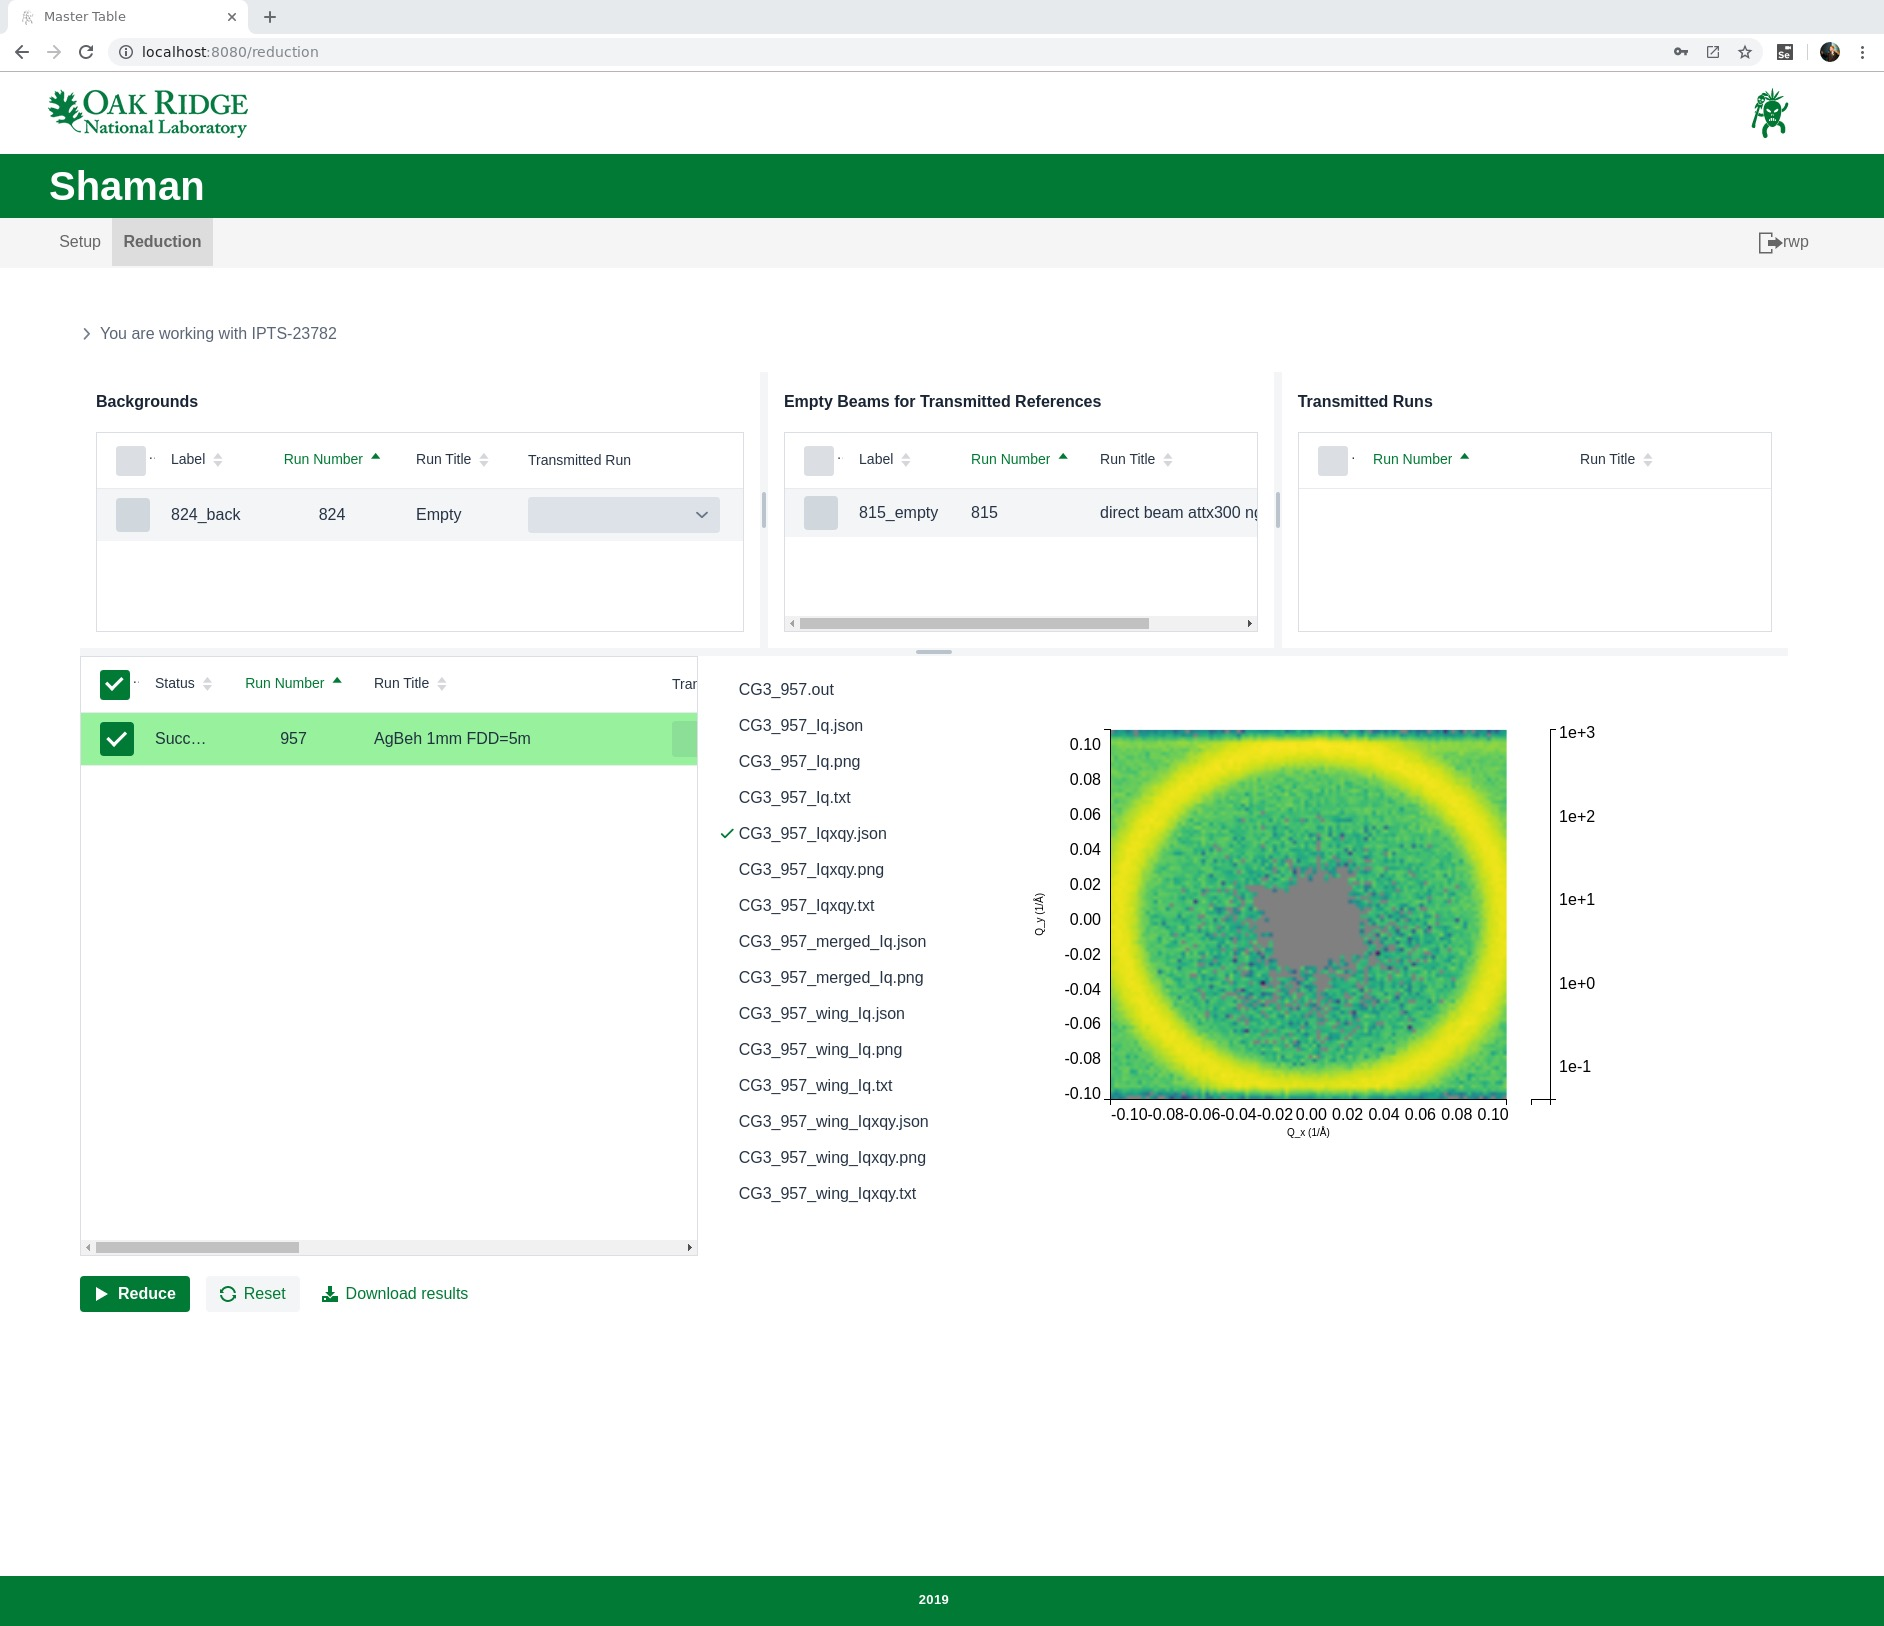
\includegraphics[width=\textwidth]{shaman-paper-2019/src/figures/biosans-IQXY.jpg}
\caption{The 2D intensity as a function of wave vector in the main BIOSANS detector as shown in Shaman.}
\label{biosans-main}
\end{figure}

\begin{figure}[htbp]
\centering
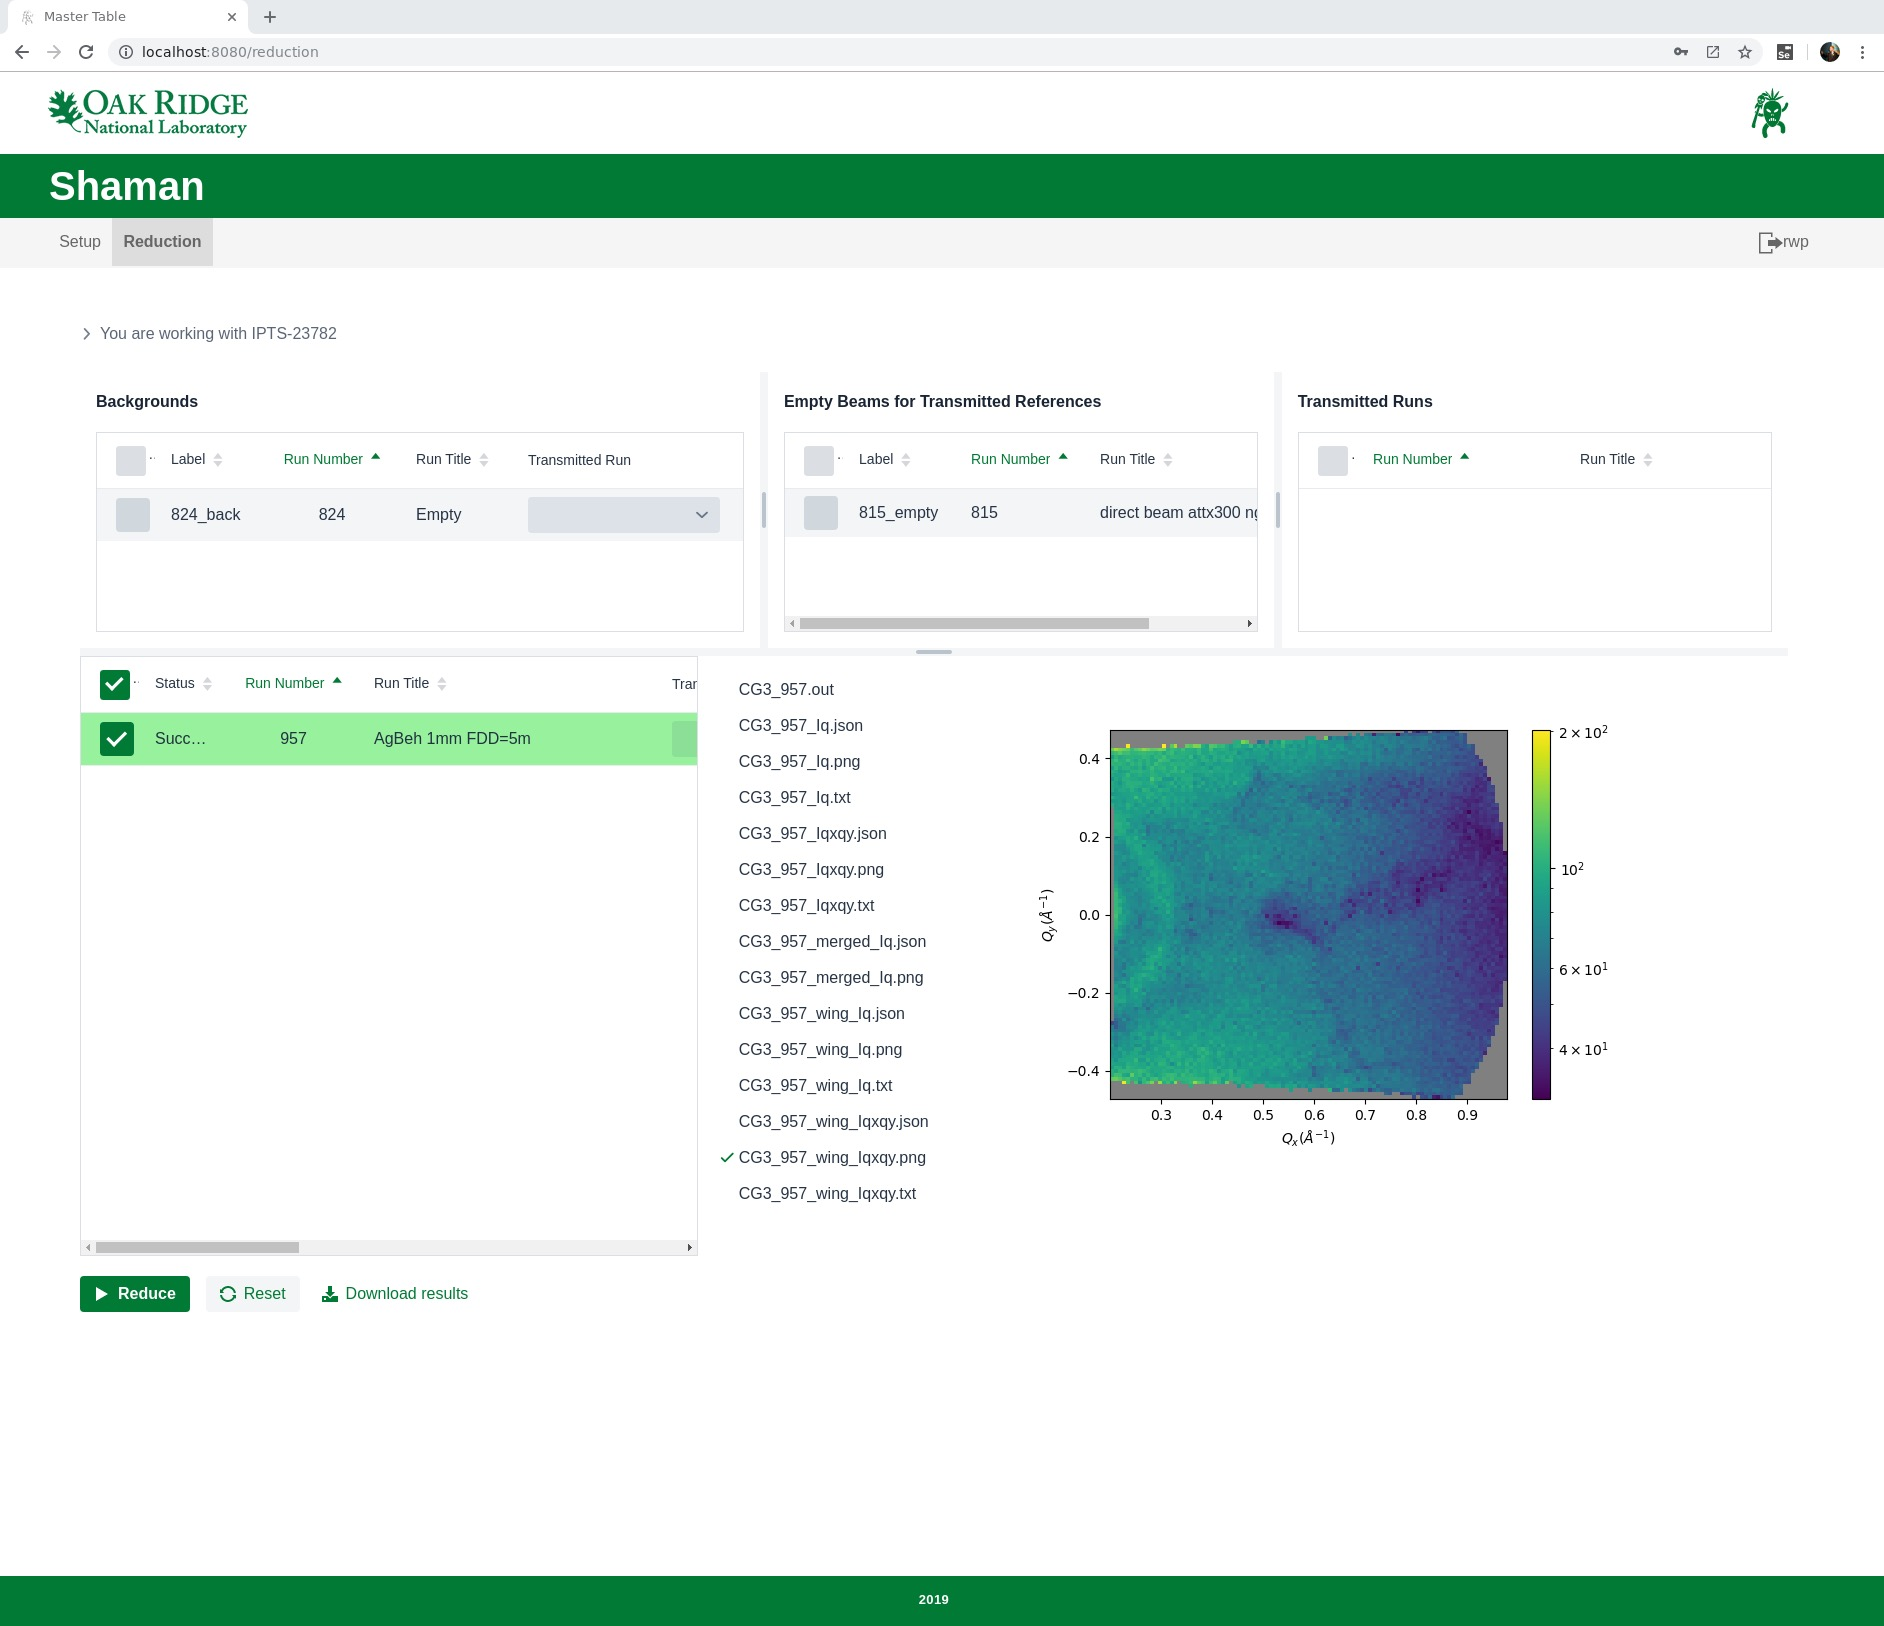
\includegraphics[width=\textwidth]{shaman-paper-2019/src/figures/biosans-IQ-wing.jpg}
\caption{The 2D intensity as a function of wave vector in the BIOSANS wing detector as shown in Shaman.}
\label{biosans-wing}
\end{figure}


Provide at least one illustrative example to demonstrate the major functions.

Optional: you may include one explanatory video that will appear next to your article, in the right hand side panel. (Please upload any video as a single supplementary file with your article. Only one MP4 formatted, with 50MB maximum size, video is possible per article. Recommended video dimensions are 640 x 480 at a maximum of 30 frames/second. Prior to submission please test and validate your .mp4 file at $ http://elsevier-apps.sciverse.com/GadgetVideoPodcastPlayerWeb/verification$. This tool will display your video exactly in the same way as it will appear on ScienceDirect.).
\section{Impact}
\label{}

\textbf{This is the main section of the article and the reviewers weight the description here appropriately}

Indicate in what way new research questions can be pursued as a result of the software (if any).

Indicate in what way, and to what extent, the pursuit of existing research questions is improved (if so).

Indicate in what way the software has changed the daily practice of its users (if so).

Indicate how widespread the use of the software is within and outside the intended user group.

Indicate in what way the software is used in commercial settings and/or how it led to the creation of spin-off companies (if so).
\section{Conclusions}
\label{}

Set out the conclusion of this original software publication.
\section{Conflict of Interest}
Please select the appropriate text:

Potential conflict of interest exists:
We wish to draw the attention of the Editor to the following facts, which may be considered as potential conflicts of interest, and to significant financial contributions to this work. The nature of potential conflict of interest is described below: [Describe conflict of interest]

No conflict of interest exists:
We wish to confirm that there are no known conflicts of interest associated with this publication and there has been no significant financial support for this work that could have influenced its outcome.
\section*{Acknowledgements}
\label{}

Optionally thank people and institutes you need to acknowledge. 

%% The Appendices part is started with the command \appendix;
%% appendix sections are then done as normal sections
%% \appendix

%% \section{}
%% \label{}

%% References:
%% If you have bibdatabase file and want bibtex to generate the
%% bibitems, please use
%%
%%  \bibliographystyle{elsarticle-num} 
%%  \bibliography{<your bibdatabase>}

%% else use the following coding to input the bibitems directly in the
%% TeX file.

\begin{thebibliography}{00}


%% \bibitem{label}
%% Text of bibliographic item

\bibitem{}

\end{thebibliography}
Please add the reference to the software repository if DOI for software  is available. 

\section*{Current executable software version}
\label{}

Ancillary data table required for sub version of the executable software: (x.1, x.2 etc.) kindly replace examples in right column with the correct information about your executables, and leave the left column as it is.

\begin{table}[!h]
\begin{tabular}{|l|p{6.5cm}|p{6.5cm}|}
\hline
\textbf{Nr.} & \textbf{(Executable) software metadata description} & \textbf{Please fill in this column} \\
\hline
S1 & Current software version & For example 1.1, 2.4 etc. \\
\hline
S2 & Permanent link to executables of this version  & For example: $https://github.com/combogenomics/$ $DuctApe/releases/tag/DuctApe-0.16.4$ \\
\hline
S3 & Legal Software License & List one of the approved licenses \\
\hline
S4 & Computing platforms/Operating Systems & For example Android, BSD, iOS, Linux, OS X, Microsoft Windows, Unix-like , IBM z/OS, distributed/web based etc. \\
\hline
S5 & Installation requirements \& dependencies & \\
\hline
S6 & If available, link to user manual - if formally published include a reference to the publication in the reference list & For example: $http://mozart.github.io/documentation/$ \\
\hline
S7 & Support email for questions & \\
\hline
\end{tabular}
\caption{Software metadata (optional)}
\label{} 
\end{table}


\end{document}
\endinput
%%
%% End of file `SoftwareX_article_template.tex'.
